\section{Пользовательский интерфейс} \label{sec:ui}
При проектировании пользовательского интерфейса учитываются понятия эргономичности и экономичности предоставляемого интерфейса.

К интерфейсу предъявляются следующие требования:
\begin{itemize}
  \item удобство, то есть способность удовлетворять требования широкого круга пользователей при решении целевых задач;
  \item понятность, то есть согласованность и очевидность обозначений и непротиворечивость описаний элементов управления;
  \item однозначность, то есть предсказуемость результатов выполняемых действий;
  \item неизбыточность, то есть отсутствие неоправданного дублирования элементов управления;
  \item простота, то есть вынесение на панели инструментов лишь необходимых элементов управления, скрытие редко используемых функций;
  \item целостность, то есть его внутренняя согласованность и единообразность.
\end{itemize}

В соответствии с приведенными требованиями, разработанный пользовательский интерфейс имеет следующий вид:
\begin{figure}[H]
  \centering
  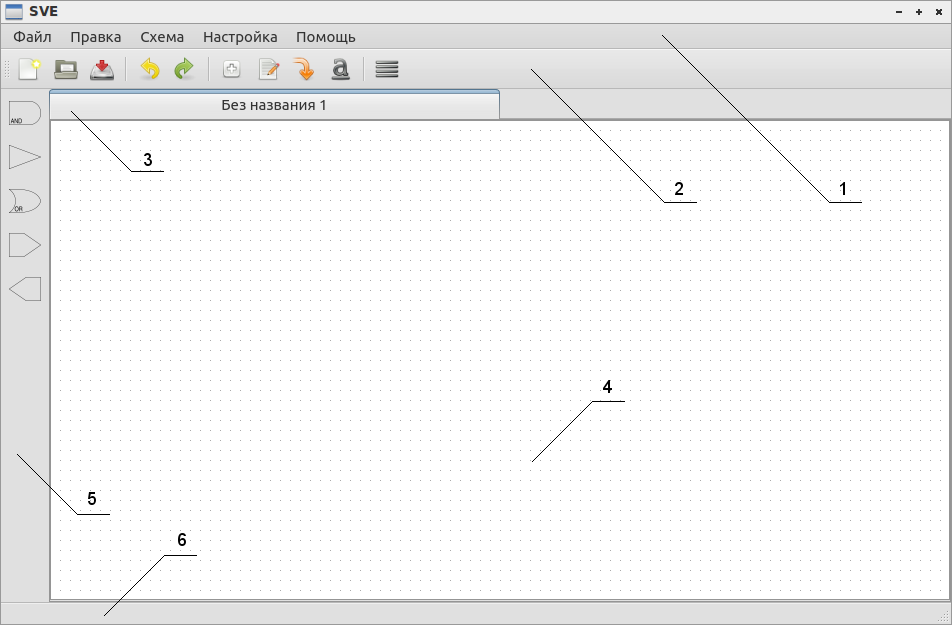
\includegraphics[width=\textwidth]{gui/main-window.png}
  \caption{Главное окно программы}
  \label{fig:main-window}
\end{figure}

Как видно из рисунка \ref{fig:main-window}, графический интерфейс программы включает:
\begin{itemize}
  \item главное меню (2)\\
  Меню <<Файл>>: содержит файловые операции, такие как создание, открытие, сохранение файлов.\\
  Меню <<Правка>>: содержит команды управления буфером обмена и историей редактирования.\\
  Меню <<Схема>>: содержит операции управления элементами схемы, позволяя добавлять узлы, связи между ними, текстовые метки, редактировать их свойства.
  Из этого же меню осуществляется просмотр VHDL-кода, описывающего схему.\\
  Меню <<Настройка>>: позволяет управлять расширениями и настройками программы.\\
  Меню <<Справка>>: содержит информацию о назначении программы, авторстве, используемых компонентах и лицензировании.
  \item основную панель инструментов (3)\\
  На эту панели вынесены наиболее часто используемые пункты главного меню: создание, открытие и сохранение файлов, отмена и повторение действий, добавление узлов, связей, меток, просмотр VHDL;
  \item переключатель рабочих областей документов (5);
  \item панель элементов (8)\\
  На нее вынесены пиктограммы элементов, загруженных из расширений;
  \item рабочую область (9)\\
  Здесь размещаются источники и приемники сигналов (1), текстовые метки (4), элементы (7), соединенные связями (6).
\end{itemize}

Управление расширениями ведется с помощью меню следующего вида, вызываемого из меню <<Настройка>> $\rightarrow$ <<Расширения>>:
\begin{figure}[H]
  \centering
  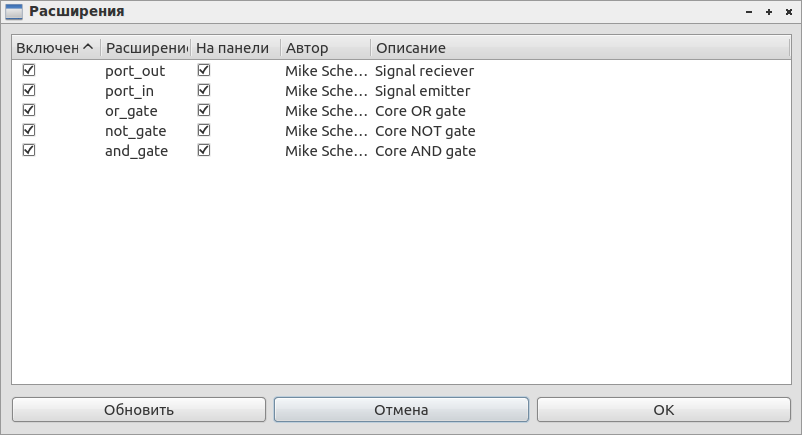
\includegraphics[width=0.9\textwidth]{gui/plugins.png}
  \caption{Управление расширениями}
  \label{fig:plugins}
\end{figure}

В окне, изображенном на рисунке \ref{fig:plugins} отображаются:
\begin{itemize}
  \item состояние расширения\\
  Если переключатель в колонке "Вкл." выставлен, то расширение будет загружено для использования в программе при следующем запуске.
  Таким образом, включение или отключение расширения требует перезапуска приложения;
  \item название расширения\\
  Этот параметр считывается из файла-описателя расширения;
  \item расположение на панели элементов\\
  Если переключатель в колонке "Акт." выставлен, то элемент будет вынесен на панель элементов (см. рисунок \ref{fig:main-window}).
  \item автор
  \item описание\\
  Примечания, указанные автором. Как и в предыдущем случае, берется из файла-описателя;
\end{itemize}

Данный список является сортируемым по всем полям.

Также присутствует кнопка "Обновить список", позволяющая принудительно перезагрузить список плагинов (например, при их добавлении).


Просмотр и редактирование VHDL осуществляется в окне, вызываемом из соответствующих пунктов меню.
\begin{figure}[H]
  \centering
  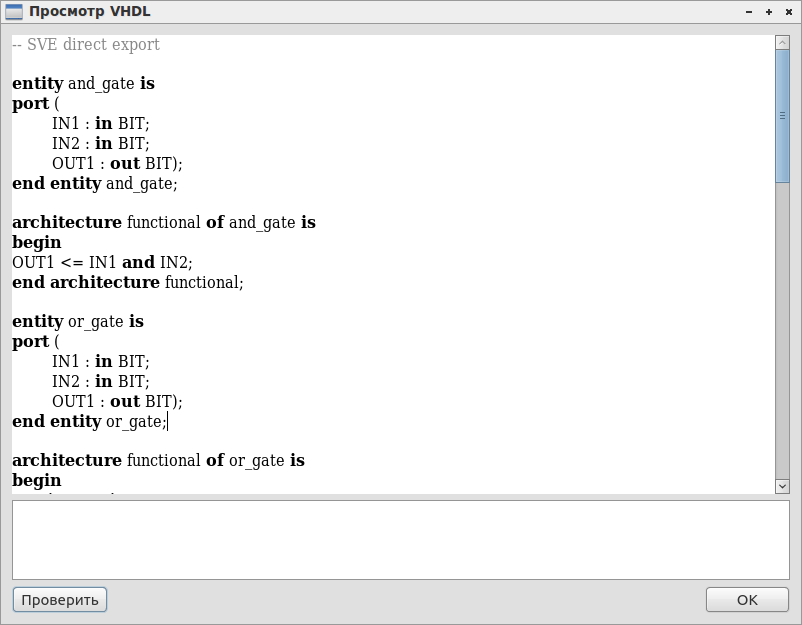
\includegraphics[width=0.6\textwidth]{gui/vhdl-view.png}
  \caption{Просмотр VHDL}
  \label{fig:vhdl-view}
\end{figure}

Как видно, при работе с исходным кодом используется подсветка синтаксических конструкций языка.